\documentclass[11pt]{article}

\usepackage{amsmath}
\usepackage{graphicx}
\usepackage{multicol}
\usepackage{natbib}
\usepackage{wrapfig}
\usepackage{hyperref}
\usepackage{tabularx}
\usepackage{setspace}
\usepackage{comment}

\usepackage[compact]{titlesec}  
\titlespacing{\section}{0pt}{0pt}{0pt}
\titlespacing{\subsection}{0pt}{0pt}{0pt}
\titlespacing{\subsubsection}{0pt}{0pt}{0pt}

\oddsidemargin 0cm
\evensidemargin 0cm

\usepackage[margin=1in]{geometry}

\parindent 0cm
\parskip 0.5cm

\usepackage{fancyhdr}
\pagestyle{fancy}
\fancyhf{}
%\fancyhead[L]{AOSS Reference Sheet}
\fancyhead[C]{\small Cyclones!}
\fancyfoot[C]{Page \thepage}

\newcommand{\vb}{\mathbf}
\newcommand{\diff}[2]{\frac{d #1}{d #2}}
\newcommand{\diffsq}[2]{\frac{d^2 #1}{{d #2}^2}}
\newcommand{\pdiff}[2]{\frac{\partial #1}{\partial #2}}
\newcommand{\pdiffsq}[2]{\frac{\partial^2 #1}{{\partial #2}^2}}
\newcommand{\topic}{\textbf}
\newcommand{\arcsinh}{\mathrm{arcsinh}}
\newcommand{\arccosh}{\mathrm{arccosh}}
\newcommand{\arctanh}{\mathrm{arctanh}}

\begin{document}

\appendix

\addtocounter{section}{3}

\section*{Notes}

- African Easterly Waves
- Why does the number of cyclones decrease in the future?  Is this robust across models (but high resolution is needed)?  Humidity at 600hPa; shearing differences?  SST distribution?
- Focus on the northern Atlantic and eastern Pacific
- Why does intensity increase?
- Are coupled model simulations needed to assess tropical cyclones?  Coupled model biases are very problematic
- Extratropical cyclones and the tropical transition.  Is the tropical transition pushed farther North?  Detection algorithm based approach to ETCs.
- An outcome is a more robust detection / stitching algorithms
- Changes in landfall?  Assessment of regions which will be more susceptible to TC damage.  How does recurving affect this?
- "Changes in global circulation and the effect on local extremes"
- Leverage the ensemble of high resolution ensemble data
- Variable resolution over the Atlantic basin; run a bunch of ensembles at 25km resolution
- What are the resolution dependencies of ETCs?
- Characterizing changing t-storms (size, wind speed, pressure, symmetry, latitude of max intensity, precipitation, latitude of maximum intensity, precipitation over land)
- Characterizing changing et-storms (size, wind speed, pressure, snow/rain precip. amounts, latitude of max. intensity)
 
\section{Project Description}

The next century will see unprecedented changes to the climate system.  These changes are particularly apparent to society through the behavior of extreme weather events. As stated in the third national climate assessment, ``changes in extreme weather and climate events, such as heat waves and droughts, are the primary way that most people experience climate change.''  Changes in such have been observed since at least 1950, and have been at least partially linked to climate change due to human influences (IPCC AR5 Synthesis Report).  In this manner, the characteristics of climate extremes are key indictors of climate change, and addressing observed and projected changes in these quantities will be crucial for future climate assessments.

The central hypotheses of this proposal are as follows:

\vspace{-0.4cm}
\begin{itemize}
\item[(H1)] Changes in African Easterly Wave activity is a driver for reduced tropical cyclone count in the Atlantic basin.

\item[(H2)] The transition point for tropical cyclones to extratropical cyclones will be pushed north in response to increased carbon dioxide and/or increased sea surface temperatures.

\item[(H3)] Point of landfall for tropical storms in both the Atlantic and Pacific basins will be pushed northward under future climate scenarios.  Overland precipitation will increase.
\end{itemize}

The \textbf{uniting themes} of this proposal are \textbf{tropical cyclones}, \textbf{extratropical cyclones}, \textbf{climate change} and \textbf{big data}: This work will drive the introduction of a high-throughput cross-validated toolset for detecting and characterizing these atmospheric phenomena in large climate datasets.  Part of the uniqueness of this proposal is that it tackles scientific questions arising from tropical cyclones and extratropical cyclones within a unified framework by considering robust event detection methods as applied in the global context.  It further considers questions of attribution and prediction by leveraging these data analysis tools and large ensemble datasets to drive the most scientifically robust conclusions.

In addition to driving the development of new methods and tools, this proposal aims for several unique and novel results.  \textbf{High-resolution model simulations} will be a major focus of this work:  Under this study, it is hypothesized that high model resolution (here considered to be grid spacings of 28km and 14km) will greatly improve the simulation of both TCs and ETCs, and will produce convergence in modeled count and intensity.  Further, it is anticipated that these features will be more realistic in the vicinity of rapidly changing topography, such as along the North American coast.  This proposal also aims to be the first to completely characterize TCs and ETCs in the \textbf{In the Community Atmopshere Model (CAM)} within the Community Earth System Model (CESM), verify that CAM produces a climatology consistent with observational data, and understand how model resolution plays a role in resolving these features.  Also the use of alternate convection schemes to model TCs and ETCs will be explored.  Finally, in addition to their mean behavior, this proposal is also interested in studying the \textbf{variability} of these features by producing and leveraging access to large ensembles of model results.

The overarching objectives of the research component of this proposal are as follows:

\begin{enumerate}
\item Develop robust methods for detection and classification of tropical cyclones and extratropical cyclones, and provide improved tools for analysis of large climate datasets.

\item Understand the influence of human-induced climate change on the characteristics of tropical cyclones and extratropical cyclones (detection and attribution) at present and in the recent past.

\item Provide a scientifically and statistically robust risk assessment in the next century for tropical cyclones and extratropical cyclones.
\end{enumerate}

The remainder of this proposal is structured as follows: Motivation is presented in section \ref{sec:Motivation}, background and ongoing work are presented in section \ref{sec:BackgroundOngoingWork}, research milestone are presented in \ref{sec:ResearchMilestones}, the integrated research and educational plan is presented in section \ref{sec:IntegratedResearchEducation} and the timeline for the proposed work is presented in section \ref{sec:Timeline}.

\subsection{Motivation} \label{sec:Motivation}

\subsubsection{Broader Impacts and Intellectual Merits}

\paragraph{Broader Impacts:}  

Landfalling TCs produce intense winds, heavy rain, high waves, and damaging storm surge in coastal locations \citep{EmanuelDivineWind}. They are currently estimated to be responsible for 19,000 fatalities per year and \$26 billion/year in damages worldwide \citep{Mendelsohn2012}, making them one of the most devastating natural phenomena.

Understanding how tropical cyclone (TC) climatology may change in the coming decades is of significant value to science and society

\paragraph{Intellectual Merits:}  

\subsection{Strengths of the team}

PI Kevin Reed brings considerable experience in high-resolution climate modeling.  His past research has focused on understanding the ability of the Community Atmosphere Model (CAM) to simulate tropical cyclones at present-day and next-generation horizontal resolution \citep{Reed2011a,Reed2011c}.  This includes the study of how tropical cyclones and precipitation extremes change with climate change using decadal climate simulations at approximately 25-km horiztonal resoluton \citep{Wehner2014,Wehner2015}. Prof Reed also has developed techniques to utilize reduced complexity testbeds for understanding cloud, circulation and precipitation sensitivities in General Circulation Models (GCMs) \citep{Reed2012a,Reed2014}. These simplified techniques have shown to be useful to rationalize robust behaviors of the Earth system and are vital to continued model development and intercomparison. Through his work, Prof. Reed has developed international collaborations in model development and high-resolution modeling.

The PI and his collaborating team are uniquely positioned to conduct multi-model ensemble intercomparisons of variable-resolution climate model output using a suite of cutting-edge atmospheric models and post-processing tools.

This project will further benefit from Co-PI Ullrich's experience with atmospheric model development  (\cite{ullrich2010high, PHLPAURDN2011SPRINGER, ullrich2012operator, ullrich2012mcore, ullrich2014fluxform, guba2014viscosity, ullrich2014understanding, ullrich2014global}), numerical analysis (\cite{ullrich2011analysis, ullrich2012considerations}) and model evaluation (\cite{DCMIP2012TESTCASES, ullrich2014proposed, kent2013dynamical, ullrich2014baroclinic}).  PI Ullrich has been heavily involved with work on variable-resolution modeling \citep{zarzycki2014aquaplanet} and adaptive mesh refinement  \citep{collins2013nonhydrostatic, mccorquodale2014adaptive}. Many relevant tools have been developed by the Co-PI, including the SQuadGen grid generation tool (described in \cite{guba2014viscosity}), the TempestRemap post-processing toolkit \citep{ullrich2015remapping} and the TempestExtremes toolkit for extreme weather detection and characterization \citep{ullrich2015extremes}. He is heavily involved in national collaborations on climate projects, and is an organizer on a number of sessions and workshops which are related to atmospheric modeling. In addition, he is closely affiliated with ongoing climate research efforts at Lawrence Berkeley National Laboratory (LBNL) and the National Center for Atmospheric Research (NCAR).

\subsection{Background and Ongoing Work} \label{sec:BackgroundOngoingWork}

The focus of this proposal is on tropical and extratropical cyclones, which will be studied in the context of climate change and big data.  Of particular interest are geographical regions surronding to the U.S., including the North Atlantic and North Pacific Ocean basins. Additional interest will be given to African Easterly Waves, as it is well known that they play a significant role in tropical cyclone formation in the North Atlantic. This proposal will bring together a number of existing technologies, datasets and studies in order to address its objectives.  These features, technologies and datasets are described below.

\subsubsection{African Easterly Waves}
African Easterly Waves are large-scale westward disturbances that originate over North Africa and are associated wight the African Easterly Jet. These tropical waves typically have wavelengths of 2000-4000 km and time periods of 3-5 days \citep{Burpee1974,Reed1977}. African Easterly Waves are traditionally thought to develop by barotropic/baroclinic instability of the African Easterily Jet \citep{Burpee1972}, but recent research suggests that convection also plays an important role in the growth and development of the disturbances \citep{Hall2006,Thorncroft2008,Hsieh&Cook2005,Berry&Thorncraft2012}. African Easterly Waves are of great importance to the formation of tropical cyclones in the North Atlantic, with over 80$\%$ of major hurricanes in the basin originating from these waves \citep{Landsea1993}. Furthermore, Eastern Pacific Ocean tropical cyclone formation is also linked to African Easterly Waves \citep{Avila&Pasch1995}. 

A number of studies have used explored African Easterly Wave activity in GCMs \citep{Ruit&DellAquila2010,Daloz2012,Skinner&Diffenbaugh2013,McCrary2014}. Recent work by \citet{Roberts2015} suggests that increased horizontal resolution improves the simulation of the tropical waves and therefore tropical cyclone counts in the North Atlantic.  Despite these studies, relatively little work has focused on the impact of climate change on the development and formation of African Easterly Waves and the connection to changes in tropical cyclones in the North Atlantic. Work by \citet{Skinner&Diffenbaugh2013}, using the CMIP5 dataset, indicates an increase in easterly wave strength (for those waves north of the African Easterly Jet), suggesting implications for the Atlantic Ocean basin. The proposed work will  further investigate how the African Easterly Wave activity behaves in higher resolution models in current and future climate, with the goal of understanding the impact of potential changes in African Easterly Wave activity on tropical cyclone in the North Atlantic.

\subsubsection{Tropical Cyclones}
Tropical cyclones (TCs) are extreme vortices that develop over the warm tropical oceans, and are among the most destructive geophysical phenomena. In the United States, tropical cyclones are the costliest of all natural disasters \citep{Pielke1998}. As a result, understanding how global and regional TC climatology will change in the coming decades is of significant value to society. Climate models are becoming a preferred tool to assess TCs in current and future climate conditions. Despite typical resolution limitations, it is well known that GCMs have the ability to simulate TCs, even at coarse horizontal resolutions of 100 km \citep{Knutson2010}. However, these simulated TCs are typically of weaker intensity and larger size than observed storms \citep{Walsh2007}. Using horizontal resolutions in the range of 10-30 km, more recent GCM studies have shown the ability to improve some of these resolution limitations \citep{Murakami2012,Manganello2012, Bacmeister2014, Wehner2014}

The general understanding is that global tropical cyclone frequency is likely to decrease, or remain relatively unchanged, with a likely increase in intensity under future climate scenarios (IPCC AR5 Synthesis Report). However, there is no consenus for the manner in which TC frequency and intensity will change regionally in a future climate using CMIP5 models \citep{Camargo2013}. The proposed research will study the attribution of anthropogenic climate change on TC intensity intensity, frequency and storm precipitation. Furthermore, the proposed work will address the questions of how climate change may impact TC climatology in the North Atlantic and North Pacific Ocean basins by making use of ensemble simulations.  

\subsubsection{Extratropical Cyclones}

Extratropical cyclones are dominant features of the mid-latitude atmosphere associated with synoptic scale low pressure systems outside the tropics \citep{serreze1995climatological}.  Similar to tropical cyclones, these systems are responsible for high winds and extreme precipitation, and consequently have the potential for large socioeconomic impact \citep{ulbrich2009extra}.  Studies of extratropical cyclones under future climate scenarios suggest that the expansion of the Hadley circulation will drive extratropical cyclones poleward \citep{bengtsson2006storm} and the warmer climate will lead to an intensification of precipitation of these storms \citep{bengtsson2009will, zappa2013multi}.  This proposal aims to address the question of attribution of changes in ETCs to anthropogenic forcing, a question which has not yet been tackled in the literature.  It will also address the issue of whether observed intensification over the southern hemisphere in reanalysis data is corroborated with model results, or is likely associated with an increase in the number of observing stations \citep{simmonds2000variability}.  Further, results from MERRA and C20C datasets (which have traditionally been neglected in favor of NCEP and ERA-40 data) will be integrated into the analysis.

\subsubsection{Global climate modeling with CESM}

The Community Earth-System Model (CESM) \cite{RBNetal2010NCAR} is a state-of-the-art Earth modeling framework developed at NCAR, consisting of atmospheric, oceanic, land and sea ice components.  This framework has been under development for nearly two decades, and has been used heavily in better understanding the effects of global climate change.  The atmopsheric component, CAM, is further broken into two components: the dynamical core, which solves the 3D primitive equations of motion for the atmosphere, and the physics parameterization suite, which incorporates processes that occur on scales finer than the model grid scale. This project will utilize simulations from two different commonly used dynamics packages. The first package, the finite-volume (FV) dynamical core based on a regular latitude--longitude grid, is built upon a 2D shallow water approach described in \citet{Lin1996,Lin1997} and is mass-conservative in flux-form. The push for high-resolution climate simulations has required that CAM be sufficiently robust to operate on horizontal scales as fine as 10 km globally, although previous generations of the dynamical cores on latitude-longitude grid have been too slow at high resolutions to operate well at these scales.  With the development of the CAM spectral element (SE) dynamical core \citep{dennis2012cam}, utilizes a continuous Galerkin method with polynomials of degree 3 to provide a fourth-order accurate horizontal discretization on a highly scalable cubed-sphere mesh.  Current experiments are only now leading to the availability of simulations on climate time-scales at 25km global resolution \citep{Bacmeister2014, Wehner2014, Wehner2015}.

\subsubsection{High-throughput event detection with TempestExtremes} \label{sec:TempestExtremes}

TempestExtremes software package, a new suite of flexible detection and characterization algorithms developed by the Co-PI for processing large climate datasets. This package uses an algorithmic framework known as ``MapReduce'' to first detect candidate events at individual times using specified criteria. Stitching is then used to track pointwise and areal detections in time. The result is a catalog of extreme weather events and associated characteristics (here treated as climate indicators) whose generation can be automated and parallelized for multiple datasets.

\begin{figure}[p]
\begin{center}
%\begin{tabular}{|p{4in}|}
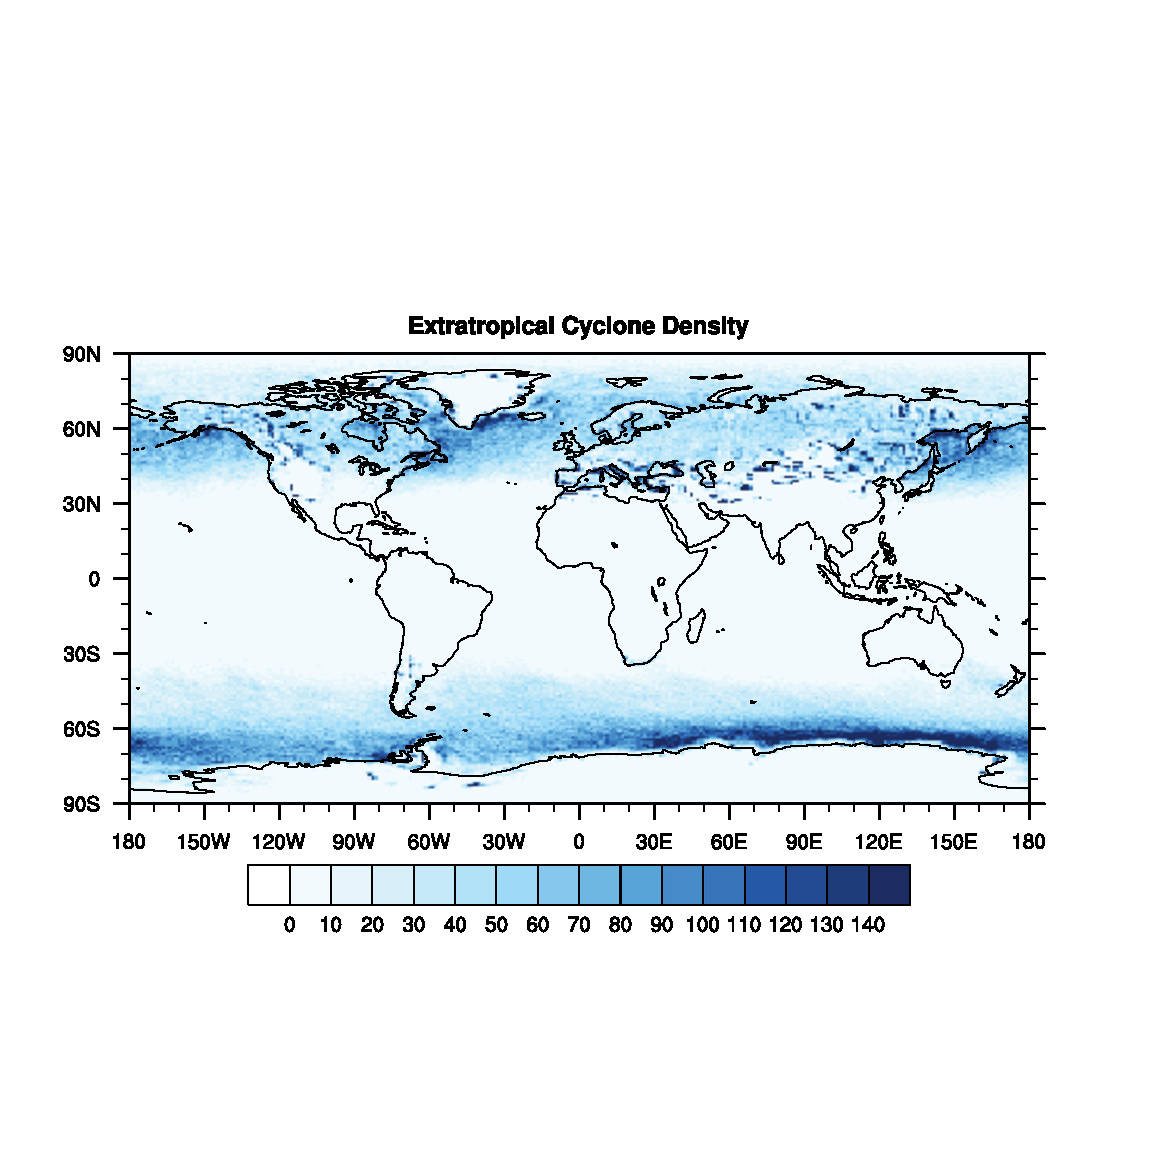
\includegraphics[trim=0.5cm 3.5cm 1cm 4.5cm, clip=true, width=4.5in]{density_plot}
\includegraphics[width=1.5in]{ETCChanges.png}
%\hline
%\end{tabular}
\end{center}
\caption{\textbf{(Left)} Example ETC counts from a 20-year CLIVAR climatological simulation, as obtained by selecting only pressure minima that (a) do not have an upper level warm core, (b) are within 4 degrees of a vorticity maximum, (c) are present over topography of maximum elevation 1500\ m, (d) are persistent for at least 2 days, (e) increase in pressure by  at least 0.1\ hPa over a distance of 1 degree in all directions, and (f) are in the latitude interval [90S, 20S] or [20N, 90N].  \textbf{(Right)} An example of differences between average annual ETC counts from a control simulation (climo) and a simulation with increased sea-surface temperatures (SSTplus2).} \label{fig:DensityPlot}
\end{figure}

In TempestExtremes, detection of both ETCs and TCs is handled by first searching for minima in the sea-level pressure field.  Thresholds can then be specified on the pointwise Laplacian of pressure, maximum or minimum latitude and topographic height at the point of detection.  Additional criteria are also available, including requirement or elimination of candidates based on the presence of a warm core aloft, the presence of a relative vorticity maximum, or the presence of a closed pressure contour.  Once candidate storms have been identified, stitching of candidates to form cyclone tracks is performed.  The stitching algorithm provides options for maximum distance between candidate points, minimum track duration, minimum distance between begin and endpoint, minimum path length, and other user-specified thresholds on quantities such as windspeed or surface pressure.  The stitching algorithm also provides an option for identifying trajectories with detection gaps, for example when candidates are present at times 1,2,3,5,6, and 7.  These criteria amalgamate a wide range of detection and stitching algorithms specified in the literature, including those criteria discussed above.  A plot of ETC densities for one possible configuration is depicted in Figure \ref{fig:DensityPlot}.  This proposal will apply this existing detection and stitching technology to the datasets in section \ref{sec:Datasets} so as to isolate historical trends of ETC and TC characteristics, and improve statistical confidence in previously observed trends.

\subsubsection{CLIVAR and Additional CAM datasets} \label{sec:CLIVAR-IPCC-CMIP5}

Climate Variability and Predictability (CLIVAR) Hurricane Working Group (HWG) experiments are  used to isolate changes in the climate system associated with accepted forcing mechanisms \citep{Walsh2015}.  Specifically, the experiments of interest for this proposal use present-day forcing which has been modified by (a) doubling atmospheric CO2 concentration (2xCO2), (b) increasing global sea-surface temperatures by 2 degrees (SST+2) or (c) a combination of (a) and (b).  CLIVAR runs have been completed using CAM over a 14-17 year integration period at 25km and a 24-27 year integration period at 100km and are now available for analysis.

Additional CAM configurations run at LBNL and NCAR will be utilized for this project. These simulations are run at approximately 25 km horizontal grid spacing near the tropics from 1980 through 2005 according to the observed Atmospheric Model Intercomparison Project (AMIP) protocols \citep{Gates1992,Gates1999} for surface temperatures, sea ice, ozone and greenhouse gases. The simulations are run with both dynamical cores, but nearly identical physical parameterization suites \citep{NCARCAM52012}. The CAM5-FV simulations have been run by Dr. Michael Wehner at LBNL. In addition to the default simulation 26-year AMIP simulation 5 additional ensemlbe simulations have been perform for 1994 to 2005. The CAM5-SE simulation have been run as part of a larger group effort at NCAR. The CAM5-SE simulations also include future time-slice experiments for 2070-2100 based on Representative Conventration Pathways (RCPs) 4.5 and 8.5 to account for future greenhouse gas forcings. 

\begin{table} 
\begin{center}
\caption{List of simulations.\label{t:runs} }
\ \\
\begin{tabular}{l c r l}
\textbf{Completed} \\
\hline
Configuration & Resolution & Length & Note \\ 
\hline
CLIVAR, CAM5-FV & 25 km & 14-17 years & 4 Different Idealized Climate Forcings  \\
AMIP, CAM5-FV & 25 km & 26 years    & 4 Additional 12-year Ensembles for 1994-2005 \\
AMIP, CAM5-SE & 25 km & 26 years    & \\
RCP4.5, CAM5-SE & 25 km & 30 years    & Time-slice 2070-2099 \\
RCP8.5, CAM5-SE & 25 km & 30 years    & Time-slice 2070-2099 \\
\hline
\\
\textbf{To Be Completed} & & & \textbf{Variable Resolution}\\
\hline
Configuration & Resolution & Length & Note \\ 
\hline
AMIP, CAM5-SE & 100$\Rightarrow$25 km & 15 years    & 5 ensembles for 1990-2005 \\
RCP8.5, CAM5-SE & 100$\Rightarrow$25 km & 15 years    & 5 ensembles for 2080-2085 \\
\hline
\end{tabular}
\end{center}
\end{table}

\subsubsection{Observation and Reanalysis products}

Reanalysis products represent climate model hindcasts which are tightly constrained to known observational data.  The importance of reanalysis products has been apparent:  Development of these products has been a major research focus, particularly over the past decade, with more than half a dozen agencies now maintaining reanalysis datasets.  However, these datasets have the potential to differ significantly depending on the choice of model, specific model parameters, the number of observations and the methodology by which data is assimilated into the model.  Although several major reanalysis products are available, this proposal aims to focus on results from NCEP \citep{kalnay1996ncep}, ERA-40 \citep{uppala2005era}, ERA-Interim \citep{simmons2007era}, MERRA \citep{rienecker2011merra} and C20C \citep{compo2011twentieth}.  For studying heat waves over the continental US, high resolution North American Regional Reanalysis (NARR) data will also be used.  The use of multiple datasets is important for identifying and overcoming biases associated with specific atmospheric models that may contaminate the results \citep{jun2008spatial}, and will lead to a set of more robust scientific conclusions.

\subsection{Research Milestones} \label{sec:ResearchMilestones}

The research milestone will be approached in a step-by-step manner as described in the following sections. A set of relevant scientific questions are also provided that will be addressed by the proposed research.

\subsubsection{Task 1a: Develop Robust Cyclone Detection and Characterization Framework}

The first main objective of the proposed research will be to develop a robust tracker for high-resolution climate model output. The tracker would allow for seamless tracking of the entire lifecycle of cyclones in the North Atlantic. This will including tracking of a tropical cyclone through extratropical transition, as well as tracing the origins of the tropical cyclone, particularly those that develop from AEWs. 

{\color{red} Why not use an existing tracker?  What modifications would you propose from the existing version of TempestExtremes?}

\subsubsection{Task 1b: Testing Detection Framework in Present-Day Climate}

Following the development cyclone framework, the algorithm will be applied to the series of the present-day AMIP CAM-FV simulation. This model dataset is choose for the validation process as it has already been well study in its ability to simulate TCs \citep{Bacmeister2014,Wehner2014} and is readily available to community. While particular interest for this proposal is to investigate the lifecycle of cyclones in the North Atlantic, the framework will be applied to the entire global dataset to ensure the vailidity of the framework in all ocean basins for future research. 

For the validation of tropical cyclones, observations from the International Best Track Archive for Climate Stewardship (IBTrACS, \citet{Knapp2010}) for the same time period (1980-2005) will be used. The comparsion will help understand biases in tropical cyclone global distribution, genesis location and intensity worldwide. \emph{Are we using reanalysis for AEWs and ETCs?}

\subsubsection{Task 2: Develop Methods for Detection and Characterization of African Easterly Waves} 

Hodges (1995) identifies a technique for tracking African Easterly waves.

{\color{red} More citations from Emily?}

Thorncroft and Hodges (2001) argue that AEWs on the southern side of the AEJ play a much greater role in tropical cyclogenesis than AEWs on the poleward side.  ``This result suggests that Atlantic tropical cyclone activity may be influenced by the number of AEWs leaving the West African coast, which have significant low-level amplitudes, and not simply by the total number of AEWs.''

Following Thorncroft and Hodges (2001), AEWs will be investigate over the latitudinal range $[5^\circ N, 15^\circ N]$ and $[5^\circ W, 25^\circ W]$.

\subsubsection{Task 3: Study Variability in Present-Day Ensemble Simulations}

Due to extreme computational costs, studies of TCs at high-resolution in climate models are typically limited to one realiztion (i.e. on esemble member). Recently however, ensemble simulation have been run in the CAM5-FV AMIP configuration for the period of 1994 to 2005 in collaboration with Michael Wehner at LBNL. The ensemble simualtions offer a unique oppurtunity to study the natural varibility of the cyclone climatology in the recent climate. In addition, the present-day climatology CAM5-FV CLIVAR simulation offers a different form of variability, as it represents the internal variability of a one year climatology runs 14-17 times. Furthermore, additional simulations using the variable-resolution cabilities of CAM5-SE will be performed to compliment the global high-resultion CAM5-SE AMIP simulations. The advantage of the variable resolution runs is that numerous ensemble runs can be performed at the same cost as the one globally uniform high-resolutiuon simulation.

\emph{How well does CAM5 perform at interannual variability?}


\subsubsection{Task 4: Investigate Climate Change Impact on Cyclone Lifecycle in the North Atlantic}

Understanding how the characteristics of tropical cyclones in the North Atlantic will change in the coming century is critical to coastal communities and the U.S. as a whole. This objective will make use of the CAM5-FV CLIVAR simulations, as well as the CAM5-SE future time-slice simulations. In addition, supplementary CAM5-SE variable resolution future simulations will be performed for this project. These additional simulations will mimic the setup proposed for present-day climate in the previous task. 

\emph{Why does the count of North Atlantic tropical cyclones decrease in future scenarios?}

Preliminary work has shown a noticeable decrease in the formation of tropical cyclones in the North Atlantic in the CAM5-SE simulations. Figure \ref{fig-rcp}, shows the track density of TCs for present-day and future simualtions using the TC detection algorithm and tracker utilized for this analysis is that used and described in \citet{Zhao2009}. The figure indicates a decrease in TCs basin-wide with the largest decrease in the eastern part of the bain off the coast of Africa. The track densities are calculated similar to \citet{Done2013} and is defined as the number of TC genesis points or tracks within a 5 degree radius of a given point per year. This pattern suggests that there is some connection between the future distribution and African easterly Waves.

Using the seamless dectection algorithm described in Task 1, this relationship between AEWs and TCs will be explored both in the idealized CLIVAR experiments and CAM5-SE simulations using the ensemble variable resolution simulations. In particular, the location and intensity of AEWs will be investigated, as well as the efficiency of the tropical waves to develop into TCs. Furthermore, a comprehensive investigation of other environmental factors, including shear, will be studied.

\emph{Is there a change in landfalling TCs?}

\emph{Is there a shift in extratopical cyclone tracks in future climate?}

In order to get a full picture of the changes in cyclones, the impact of increase radiative forcing on ETCs is also proposed. This task will focus on shifts in ETCs regions of formation, including those that develop from TCs, as well as overall changes in track distribution and intensity. \emph{Should we types of transition... I'm thinking of Superstorm Sandy?}

\subsubsection{Task 5:}

\subsection{Online access to climate data and results}

Dissemination of climate data and scientific results is an important issue for increasing public understanding of climate change.  To this end, the PI will work to develop a website (via the domain \url{http://climate.ucdavis.edu}) which allows for easy access to the results of the research component of this proposal, as well as other results that draw from existing climate data.  This webspace would allow for users to query the database of climate data, and would provide frequent and accessible commentary on the latest results to emerge from the climate science community.  The PI's past experience as a professional web developer and experience with HTML and PHP will be advantageous to the development of this project.

\subsection{Timeline} \label{sec:Timeline}

Each of the graduate student researchers involved in this project will work on one of the atmospheric features presented in this proposal: either tropical cyclones events or extratropical cyclones, although it is anticipated that there will be substantial collaboration on the technical level.  Each year of the proposal is expected to be approximately associated with one task as described in section \ref{sec:ResearchMilestones}.  The approximate timeline, including components of the educational plan, is as follows:

\begin{tabularx}{\textwidth}{cX}
\hline
\textbf{Year 1} & $\cdot$ Develop and test cyclone detection framework. \\
& $\cdot$ Begin validation of framework on CAM5-FV model dataset.  \\
& $\cdot$ Setup and start CAM5-SE present-day and RCP8.5 variable resolution ensemble runs. \\
\hline
\textbf{Year 2} & $\cdot$ Finalize framework validation using CAM5-FV. \\
& $\cdot$ Write overview article introducing lifecycle detection framework .\\
& $\cdot$ Complete CAM5-SE present-day and RCP8.5 variable resolution ensemble runs. \\
& $\cdot$ Complete analysis on varibility using CAM5-FV and CAM5-SE ensemble simulations. \\
\hline
\textbf{Year 3} & $\cdot$ Write journal article on North Atlantic cyclone variability. \\
& $\cdot$ Complete analysis of future climate simulations. \\
& $\cdot$ Write journal article on North Atlantic cyclone activity in future climate. \\
\hline
\end{tabularx}

We anticipate that multiple major peer-reviewed publications will arise from this work, addressing the studies of detection, attribution and prediction. Further, this work will be presented at major scientific meetings, including the annual meetings for the American Meteorological Society, the European Geophysical Union and the American Geophysical Union.

{\setbox0\vbox{\bibliography{mybib}}}
\bibliographystyle{wileyqj}

\end{document}
